% File: background.tex
% Date: 8.27.2014
% Author: Jared Bold

\chapter{Background}

% Hardware
\section{Hardware - Xilinx ZC702}

The hardware platform selected is the Xilinx ZC702 Evaluation Board, based around the Xilinx Zynq XC7Z020-1CLG484C. The board provides many standard peripherals such as 1 GB DDR3 RAM, 128 Mb QSPI flash memory, USB 2.0 transceiver, SD Card interface, USB JTAG interface, HDMI, Ethernet PHY with RJ-45 connector, and additional peripherals and user I/O as shown in Figure \ref{fig:zc702_top_level} \cite{xilinx_zc702}.  The purpose of the evaluation board is primarily to allow for a system design to be tested prior to producing a custom board layout, and makes it an ideal development platform for this work.

\begin{figure}[!h]
  \centering
  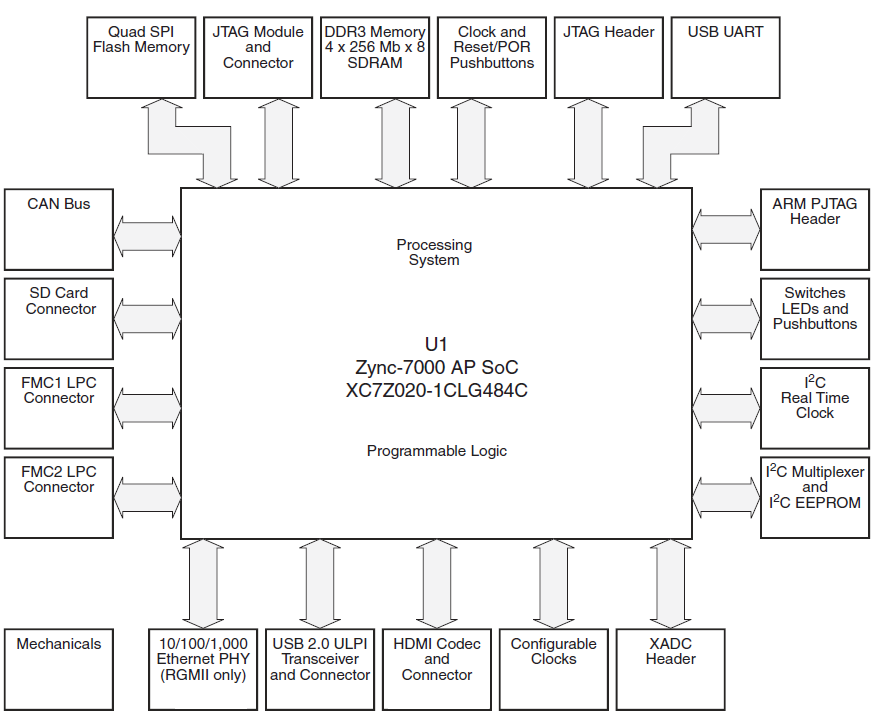
\includegraphics[width=0.9\textwidth]{./img/zc702_top_level.PNG}
  \caption{Top-Level Diagram of Xilinx ZC702 Evaluation Board}
  \label{fig:zc702_top_level}
\end{figure}

The Xilinx Zynq XC7Z020-1CLG484C device combines a Processing System (PS) and Programmable Logic (PL) on the same chip, forming a System on a Chip (SoC).  The PS is comprised of two ARM Cortex-A9 MPCore application processors (APUs), each containing a NEON co-processor, a 32 KB L1 instruction cache, and a 32 KB L1 data cache.  The APUs share a common 512 KB L2 cache.  The PL is designed using the Xilinx Artix-7 fabric, their middle-grade fabric, with 85K Logic Cells (LCs), 53,200 Look-Up Tables (LUTs), 106,400 Flip-Flops (FFs), 560 KB Block RAM, and 220 DSP Blocks \cite{xilinx_zynq}. Figure \ref{fig:zynq_top_level} shows the top level view of the composition of the Zynq device.  Communication between the two portions of the chip occurs via a subset of the communication buses specified by the Advanced Microcontroller Bus Architecture (AMBA), known as the Advanced eXtensible Interface (AXI).  The PL can be user programmed to provide access to additional peripherals or to offload processing from the APUs.

\begin{figure}[!h]
  \centering
  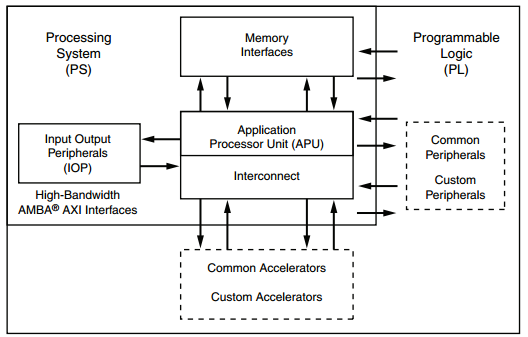
\includegraphics[width=0.9\textwidth]{./img/zynq_top_level.PNG}
  \caption{Top-Level Diagram of Xilinx Zynq device}
  \label{fig:zynq_top_level}
\end{figure}

The reason the ZC702 was selected is two-fold.  The first being the use of the Xilinx Zynq device, which provides an ideal environment for building and testing homogeneous processing environments without limitations of using separate CPU and FPGA chips.  Secondly, the Zynq device and the ZC702 board have a large amount of support from the open source community.  The wealth of information and example code provide an excellent starting place.

% Operating System
\section{Operating System - Linux 3.14}

For purposes of this work, the Linux operating system has been selected to run on the ZC702 evaluation board.  This Linux kernel is compiled directly from source maintained by Xilinx and is based off of the mainstream Linux kernel 3.14.  The Linux kernel separates the operating system into two distinct spaces, the User Space and the Kernel Space.  User applications run in the User Space and use calls to the system call interface and the GNU C Library to communicate and interact with the Kernel Space, as shown in \ref{fig:linux_kernel}.  In the Kernel Space, system resources such as memory and peripherals are accessible and can be interacted with.  The memory seen within the User Space is known as a virtual memory space which maps to a physical memory in the Kernel Space.  The Linux kernel provides several features including process management, memory management, a virtual file system, a network stack, and device drivers \cite{ibm_linux_kernel}.  These features allow for easier development and interaction between User Space applications and the hardware running underneath.

\begin{figure}[!h]
  \centering
  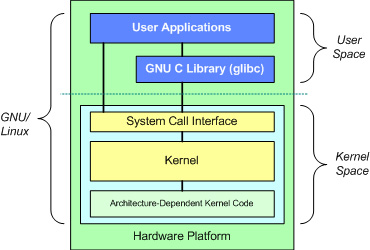
\includegraphics[width=0.9\textwidth]{./img/linux_kernel.png}
  \caption{View of Linux kernel}
  \label{fig:linux_kernel}
\end{figure}

Using Linux has several advantages over writing a bare-metal application.  One of the greatest benefits comes from the portability and ease of access to both development tools and open source applications.  An application that had previously been compiled for a Linux operating system can be recompiled to run in the embedded environment.  These applications can range from image processing libraries (LibTiff) to communications (ssh) to file transfer (ftp) to any number of other things.  The tools needed to do this, such as gcc, are readily available and open source, making them free to use.  In addition to applications, Linux provides device drivers for much of the hardware in use today, and if a driver does not exist, one can be created based on an existing driver allowing for easy access and interaction with hardware peripherals.  This is of great benefit when compared with having to write to device registers by hand in a bare-metal application.

In addition to device drivers, the Linux kernel provides a method of directly mapping physical memory in the Kernel Space to virtual memory in a User Space application using the mmap system call.  This proves very useful in SoC applications where the peripherals are memory mapped and may change based on the configuration of the device.  Using this mapping, the registers of an external device can be directly written to from the User Space, bypassing the need to develop a custom device driver and allowing for faster development and testing.

% AXI Standards
\section{Advanced Microcontroller Bus Architecture}
Central to the design of heterogeneous systems is the necessity to move data between the different processing units of the SoC.  In order to facilitate this, ARM has developed a set of specifications known as the Advanced Microcontroller Bus Architecture (AMBA) which consists of a number of protocols and interfaces to allow for the efficient movement of such data based on a Master/Slave relationship using a Ready/Valid handshake.  The Zynq device supports a number of memory-mapped interfaces for communication between the PS and PL including two 32-bit Advanced eXtensible Interface (AXI) master interfaces, two 32-bit AXI slave interfaces, four 32/64-bit hit performance AXI ports for direct access to DDR, and one 64-bit AXI slave interface known as the Accelerator Coherency Port (ACP).  While the memory-mapped interfaces allow for data to be easily transferred into and out of the PL, a method of easily streaming data through the PL for processing is also provided by the AXI streaming interface.  Using IP developed around the AXI stream protocol, different processing blocks are easily linked together to form a processing pipeline.  Figure \ref{fig:axi_pipeline} shows an example processing pipeline utilizing both the memory-mapped and streaming AXI interfaces.  Xilinx provides a number of IP cores to be used in hardware development to interface with both memory-mapped and streaming AXI interfaces.

\begin{figure}[!h]
  \centering
  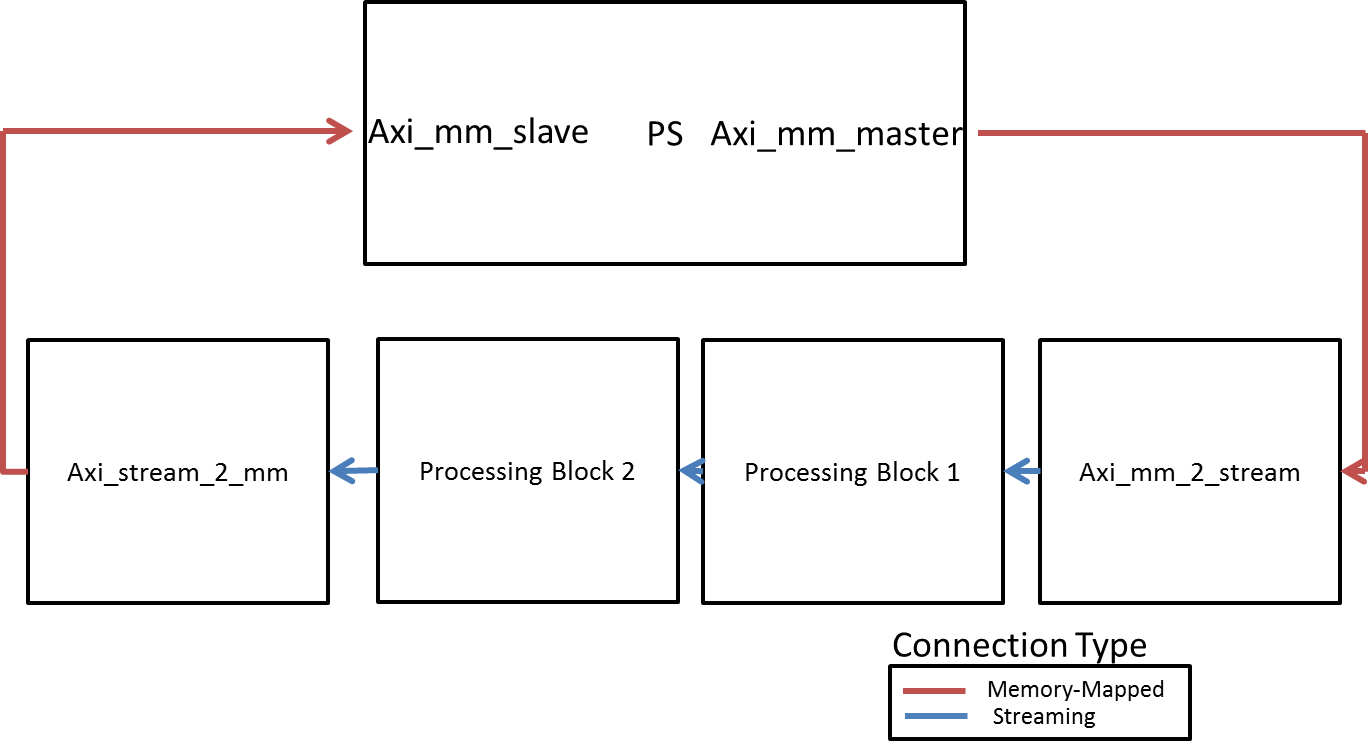
\includegraphics[width=0.9\textwidth]{./img/axi_pipeline.png}
  \caption{Example AXI processing pipeline}
  \label{fig:axi_pipeline}
\end{figure}

\section{Image Filtering}
Image filtering is a core operation in the field of image processing.  It is the process of subjecting an input image to a linear, space invariant (LSI) system resulting in an output image that is the convolution of the input and the LSI system, in this case the filter kernel \cite{jain1995machine}.  The filter kernel is a matrix of coefficients that when convolved with the input image results in a weighted sum of the current pixel and neighboring pixels, which is then stored in the output image.  Figure \ref{fig:filter_example} shows an example of how a filter kernel would be applied.  Due to the nature of convolution, the kernel must be flipped about the horizontal and vertical axis prior to being applied to the input image and calculating the output.
\begin{figure}[!h]
  \centering
  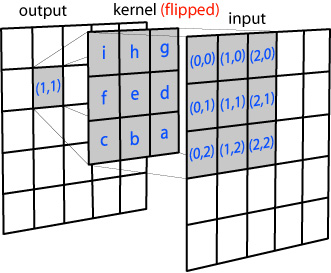
\includegraphics[width = 0.5\textwidth]{./img/filter_example.jpg}
  \caption{Image filtering example}
  \label{fig:filter_example}
\end{figure}

The process of filtering an image can become increasingly resource intensive as the size of the kernel increases.  For the example shown in \ref{fig:filter_example}, a single output pixel would be calculated using equation \eqref{eq:filter_eq1}.
\begin{equation}
  \begin{split}
  O(1,1) =& I\times I(0,0)+H\times I(1,0)+G\times I(2,0)+ \\
          &F\times I(0,1)+E\times I(1,1)+D\times I(2,1)+ \\
          &C\times I(0,2)+B\times I(1,2)+A\times I(2,2)
  \label{eq:filter_eq1}
  \end{split}
\end{equation}
In order to reduce the computational load, symmetric filters are typically used of the format shown in \ref{fig:filter_symmetric}. A filter of this form has an output pixel equation given by \eqref{eq:filter_symmetric}.
\begin{equation}
  \begin{split}
    O(1,1) =& A\times I(1,1)+ \\
            &B\times \left(I(0,1)+I(1,0)+I(2,1)+I(1,2)\right) +  \\
            &C\times \left(I(0,0)+I(2,0)+I(0,2)+I(2,2)\right)
  \label{eq:filter_symmetric}
  \end{split}
\end{equation}
A comparison of the number of computations between the different sized filters and their symmetric counterparts, shown in table \ref{tbl:filter_ops}, shows the benefit of using symmetric filters.
\begin{figure}[h]
  \centering
  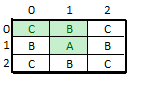
\includegraphics{./img/filter_3x3_template.PNG}
  \caption{Symmetric Filter}
  \label{fig:filter_symmetric}
\end{figure} 

\begin{table}[h]
  \begin{tabular}{|c||c|c|c|}
    \hline 
    Filter Type & Additions & Multiplications & Computational Load \\ \hline \hline
    3x3 Filter &  8 & 9 & 100\%\\ \hline
    9x9 Filter & 80 & 81 & 100\% \\ \hline
    3x3 Symmetric Filter & 8 & 3 & 64.7\% \\ \hline
    9x9 Symmetric Filter & 80 & 15 & 59.0\% \\ \hline
  \end{tabular}
  \caption{Operations required for different filter kernels}
  \label{tbl:filter_ops}
\end{table}

\section{Bilinear Interpolation}
Bilinear interpolation (BI) is the process by which an unknown value is interpolated based on a 2 dimensional interpolation process using 4 known values.  In its application in image processing, BI is used to scale images up and down.  Unlike nearest-neighbor interpolation, which relies on only one known value resulting in blocky images, BI has creates smoother images when scaling due to its estimation of intermediate values.

\begin{figure}[ht]
  \centering
  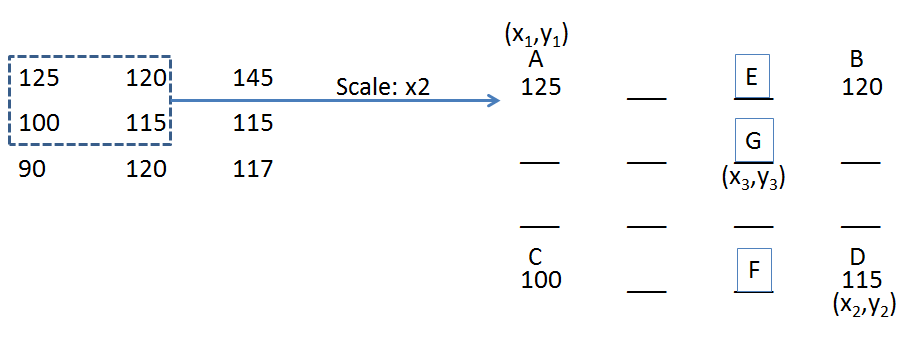
\includegraphics[width=0.9\textwidth]{./img/bilinear_example.PNG}
  \caption{Bilinear Interpolation of Grayscale Image}
  \label{fig:bilinearExample}
\end{figure}
The process of bilinear interpolation begins by expanding the known pixels to their scaled locations.  This expansion process generates a window of unknown pixels, bounded by four corners of known pixels, as shown in \ref{fig:bilinearExample}.  In order to calculate the the unknown pixel values, three equations must solved.  To generate an final equation for the value, the variables shown in \ref{fig:bilinearExample} will be used.  The first equation is the horizontal interpolation of the value at $E$.
\begin{equation}
  E = \frac{x_3-x_1}{x_2-x_1}B + \frac{x_2-x_3}{x_2-x_1}A
  \label{eqn:E}
\end{equation}
Next, the horizontal interpolation of the value at $F$ is calculated.
\begin{equation}
  F = \frac{x_3-x_1}{x_2-x_1}D + \frac{x_2-x_3}{x_2-x_1}C
  \label{eqn:F}
\end{equation}
Finally, the vertical interpolation of value at $G$ is calculated.
\begin{equation}
  G = \frac{y_3-y_1}{y_2-y_1}F + \frac{y_2-y_3}{y_2-y_1}E
  \label{eqn:G}
\end{equation}

\begin{equation}
  \alpha = x_3 - x_1, 
  \beta = x_2 - x_3, 
  \gamma = y_3 - y_1, 
  \omega = y_2 - y_3
  \label{eqn:rename}
\end{equation}
By substituting \eqref{eqn:E} and \eqref{eqn:F} into \eqref{eqn:G} and allowing variables to be renamed as in \eqref{eqn:rename}, the BI equation for a pixel is determined.
\begin{equation}
  G = \frac{1}{(\omega + \gamma)(\beta + \alpha)}[\gamma(\alpha D + \beta C) + \omega(\alpha B + \beta A)]
  \label{eqn:bilinear}
\end{equation}

By applying \eqref{eqn:bilinear} to every unknown pixel in every window that is generated from the scaling process, an image is enlarged or shrunk with minimal loss of quality.  This technique is easily extended to multiple color channel images such RGB by operating on each color plane individually and ensuring that pixel offsets are correctly calculated.
